%****************************************************************************%
%* Ganglia Module                                                           *%
%*                                                                          *%
%* Author(s):                                                               *%
%* - Abdelkader AMAR (Abdelkader.Amar@ens-lyon.fr)                          *%
%* - David LOUREIRO (David.Loureiro@ens-lyon.fr)                            *%
%*                                                                          *%
%* $LICENSE$                                                                *%
%****************************************************************************%
%* $Id: GUM_Ganglia.tex,v 1.2 2007/11/29 16:03:21 dloureir Exp $
%* $Log: GUM_Ganglia.tex,v $
%* Revision 1.2  2007/11/29 16:03:21  dloureir
%* typo corrections
%*
%* Revision 1.1  2007/11/08 16:53:48  dloureir
%* Adding the ganglia part in the User's Manual
%*
%* Revision 1.2  2007/11/08 11:31:14  dloureir
%* Correcting the headers
%*
%****************************************************************************%
\chapter{The Ganglia module for \grudu}

\section{Ganglia short introduction}

Ganglia is a scalable distributed monitoring system for high-performance
computing systems such as clusters and Grids. It is based on a hierarchical
design targeted at federations of clusters. It leverages widely used
technologies such as XML for data representation, XDR for compact, portable
data transport, and RRDtool for data storage and visualization. It uses
carefully engineered data structures and algorithms to achieve very low
per-node overheads and high concurrency. The implementation is robust, has been
ported to an extensive set of operating systems and processor architectures,
and is currently in use on thousands of clusters around the world. It has been
used to link clusters across university campuses and around the world and can
scale to handle clusters with 2000 nodes.          

Ganglia is an open-source project that grew out of the University of
California, Berkeley Millennium Project which was initially funded in large
part by the National Partnership for Advanced Computational Infrastructure
(NPACI) and National Science Foundation RI Award EIA-9802069. NPACI is funded
by the National Science Foundation and strives to advance science by creating a
ubiquitous, continuous, and pervasive national computational infrastructure:
the Grid. Current support comes from Planet Lab: an open platform for
developing, deploying, and accessing planetary-scale services.       

You can find more information on the Ganglia Website at
\url{http://ganglia.sourceforge.net} 

\section{Ganglia plugin}

As Ganglia is installed on \gfk, the \grudu users can have access to the
information provided by the software inside \grudu.

If you selected the ganglia plugin during the installation step of \grudu, there
is two ways to use it:
\begin{itemize}
  \item From the site information panels, where you can have instantaneous
  low-level information about every nodes of the site (computation nodes but also
  frontends).
  \begin{figure}[H]
  \centering 
  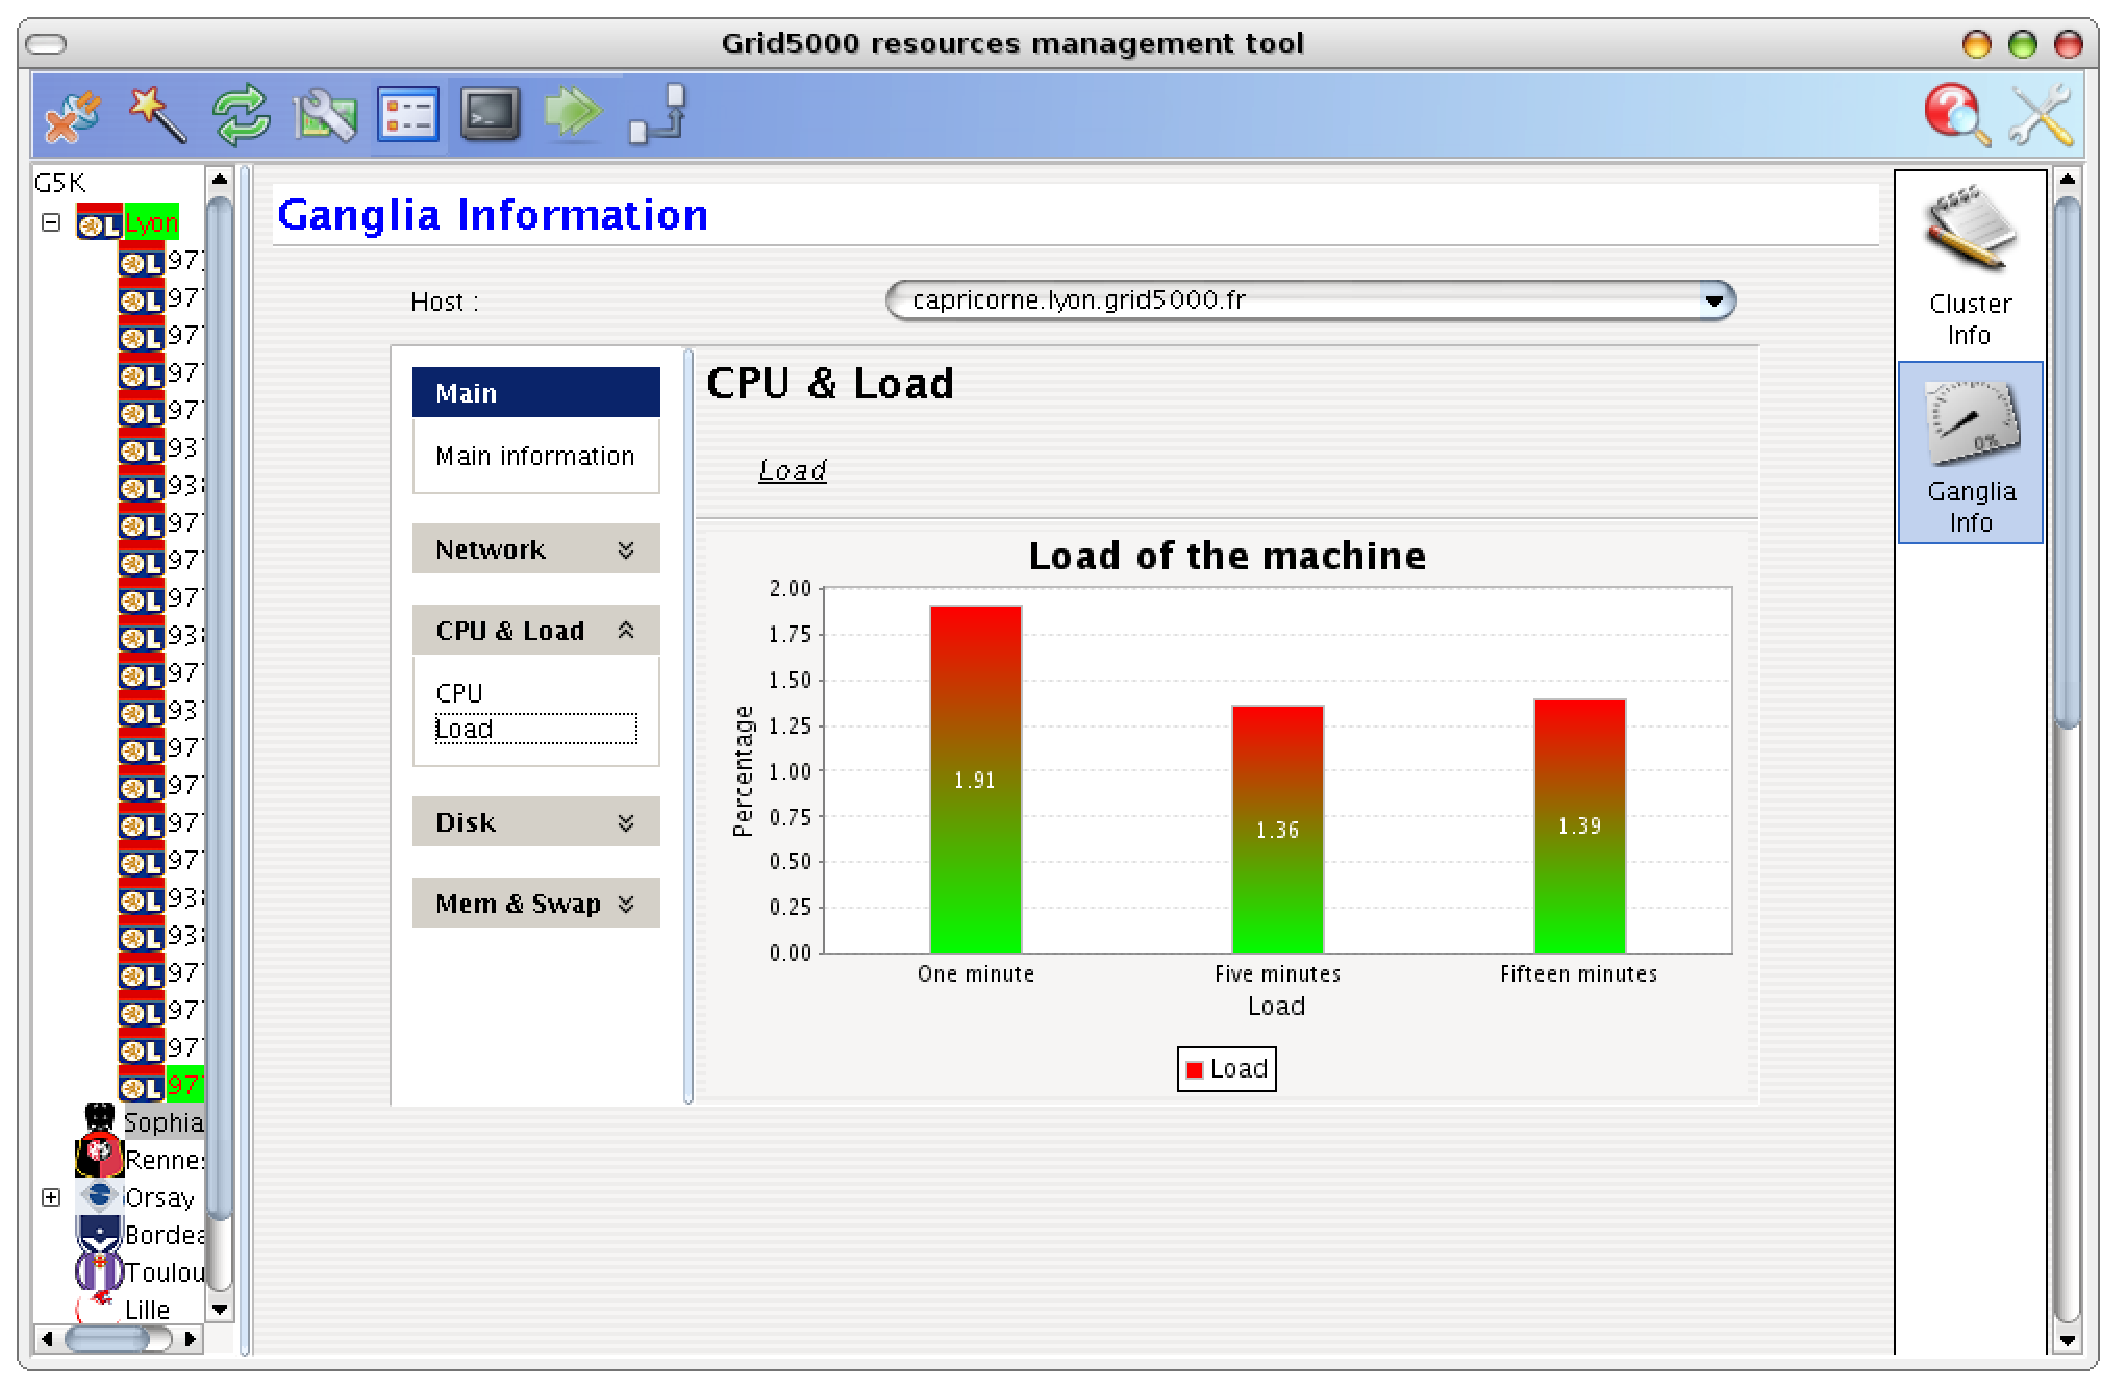
\includegraphics[width=0.5\linewidth]{figures/GRUDU_interface3_ganglia.eps}
	\caption{Ganglia plugin for the site view}
	\label{fig:GRUDU_view_site_ganglia}
  \end{figure}
  \item From the job information panels, where you can get the history of the
  low-level information brought to you by Ganglia. Concerning the generation of
  the history you have first to configure the history generation, which means defining:
  \begin{description}
  \item the period of data refreshing (of the form : hh:mm:ss)
  \item the range of the chart (same format)
  \item the path to the java home on the main node of your reservation for the
  launch of the remote jar creating the history.
  \end{description}
  \begin{figure}[H]
  \centering
  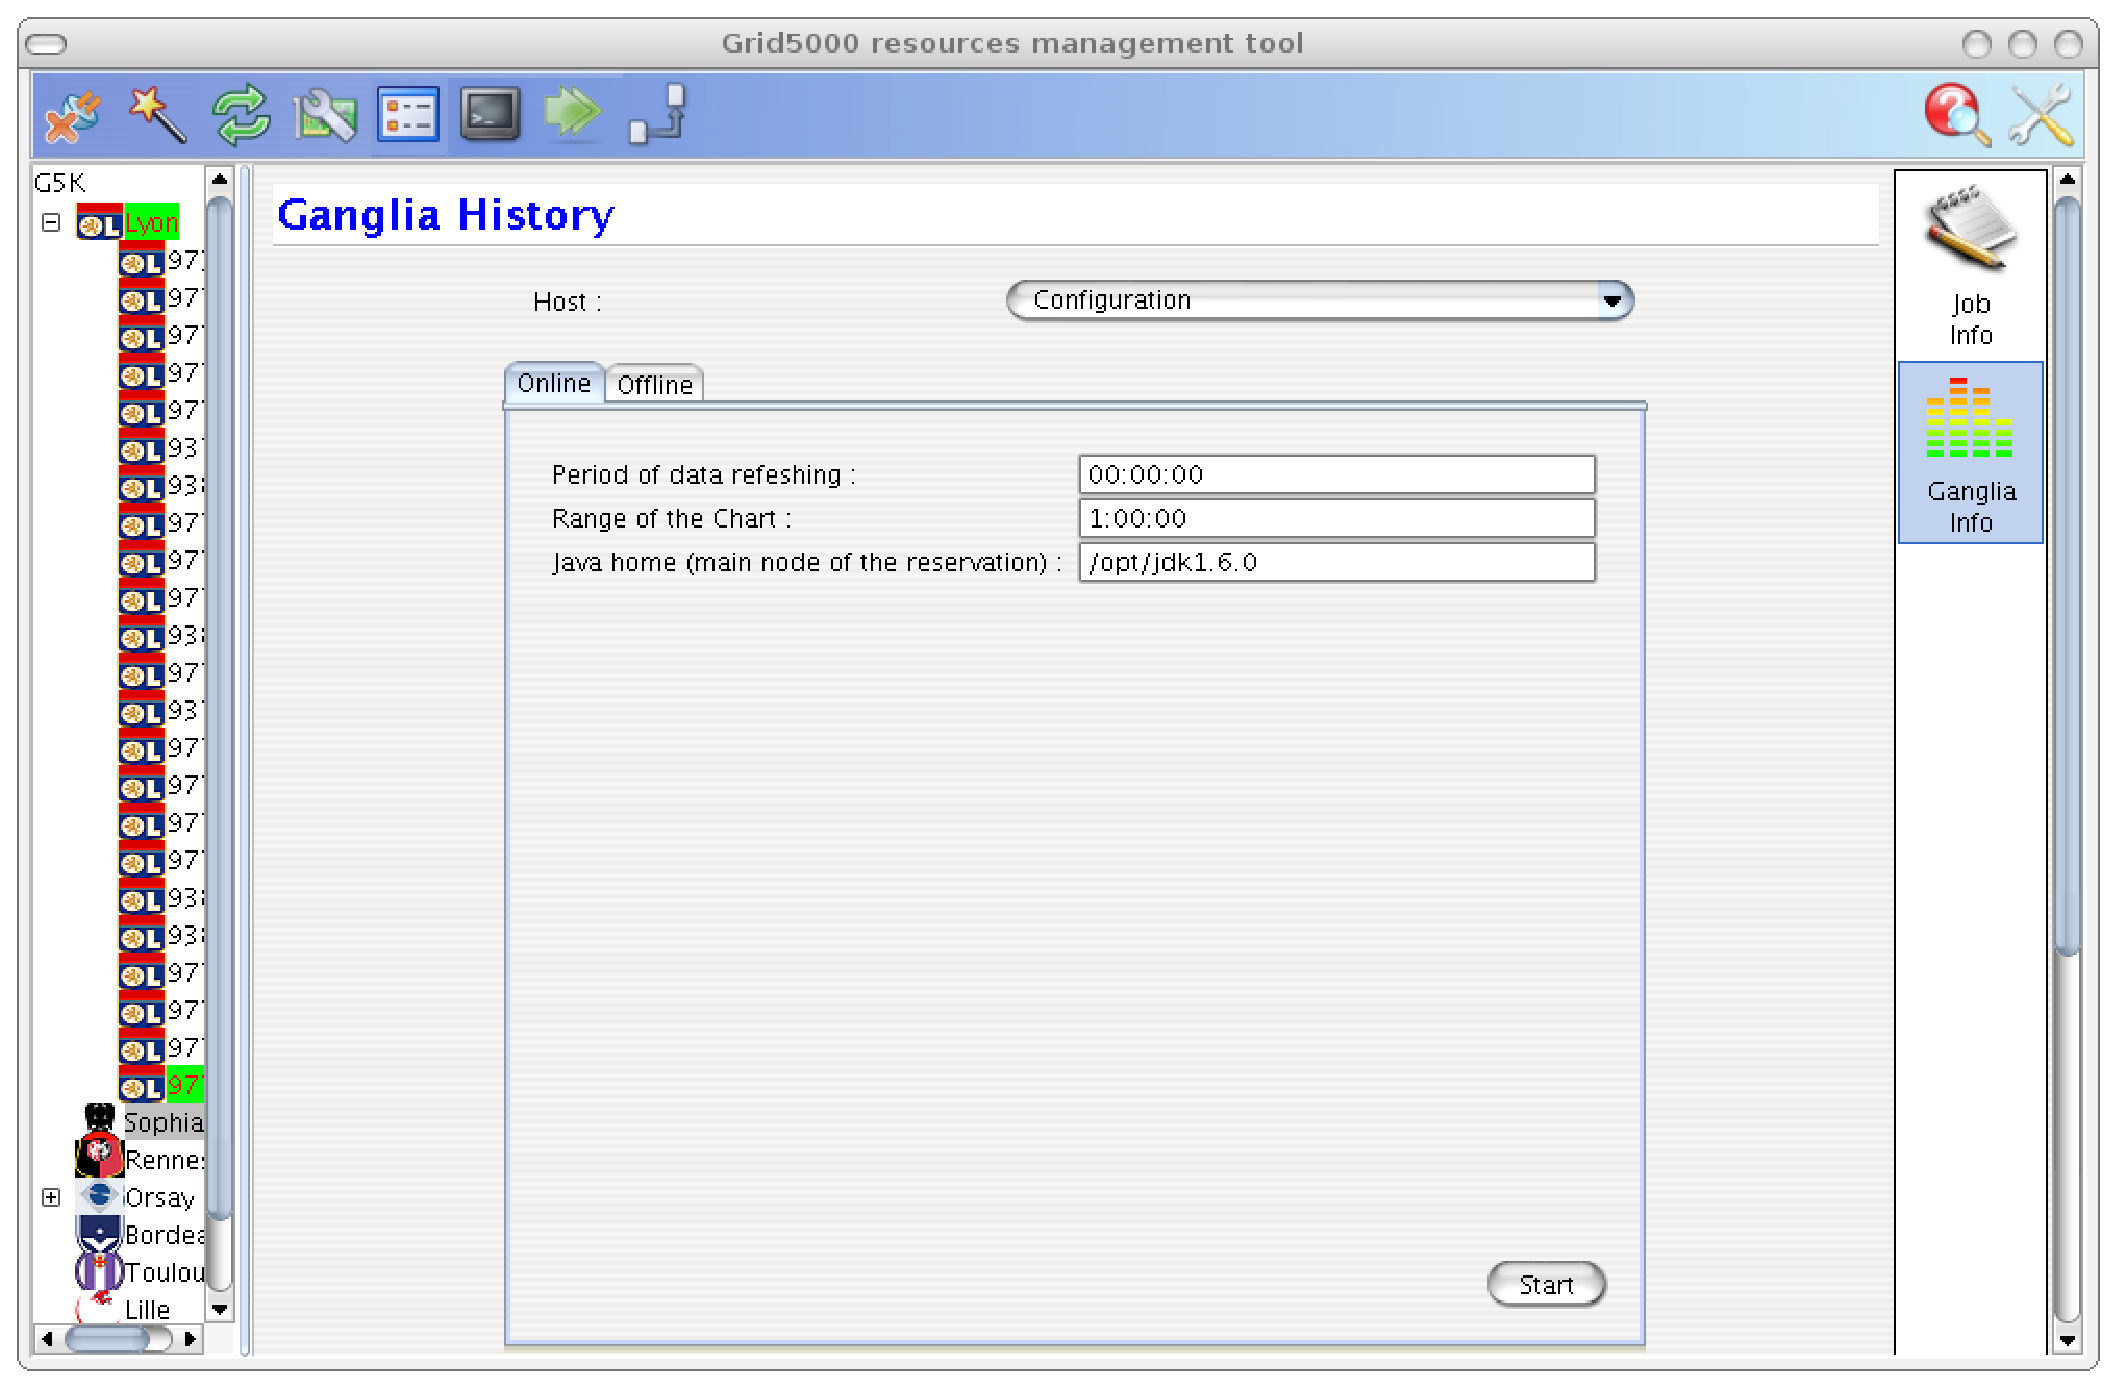
\includegraphics[width=0.5\linewidth]{figures/GRUDU_interface4_ganglia_prerequisites.eps}
  \caption{Configuration of the Ganglia plugin for the job view}
	\label{fig:GRUDU_view_job_ganglia_prerequisites}
  \end{figure}
  \begin{figure}[H]
  \centering
  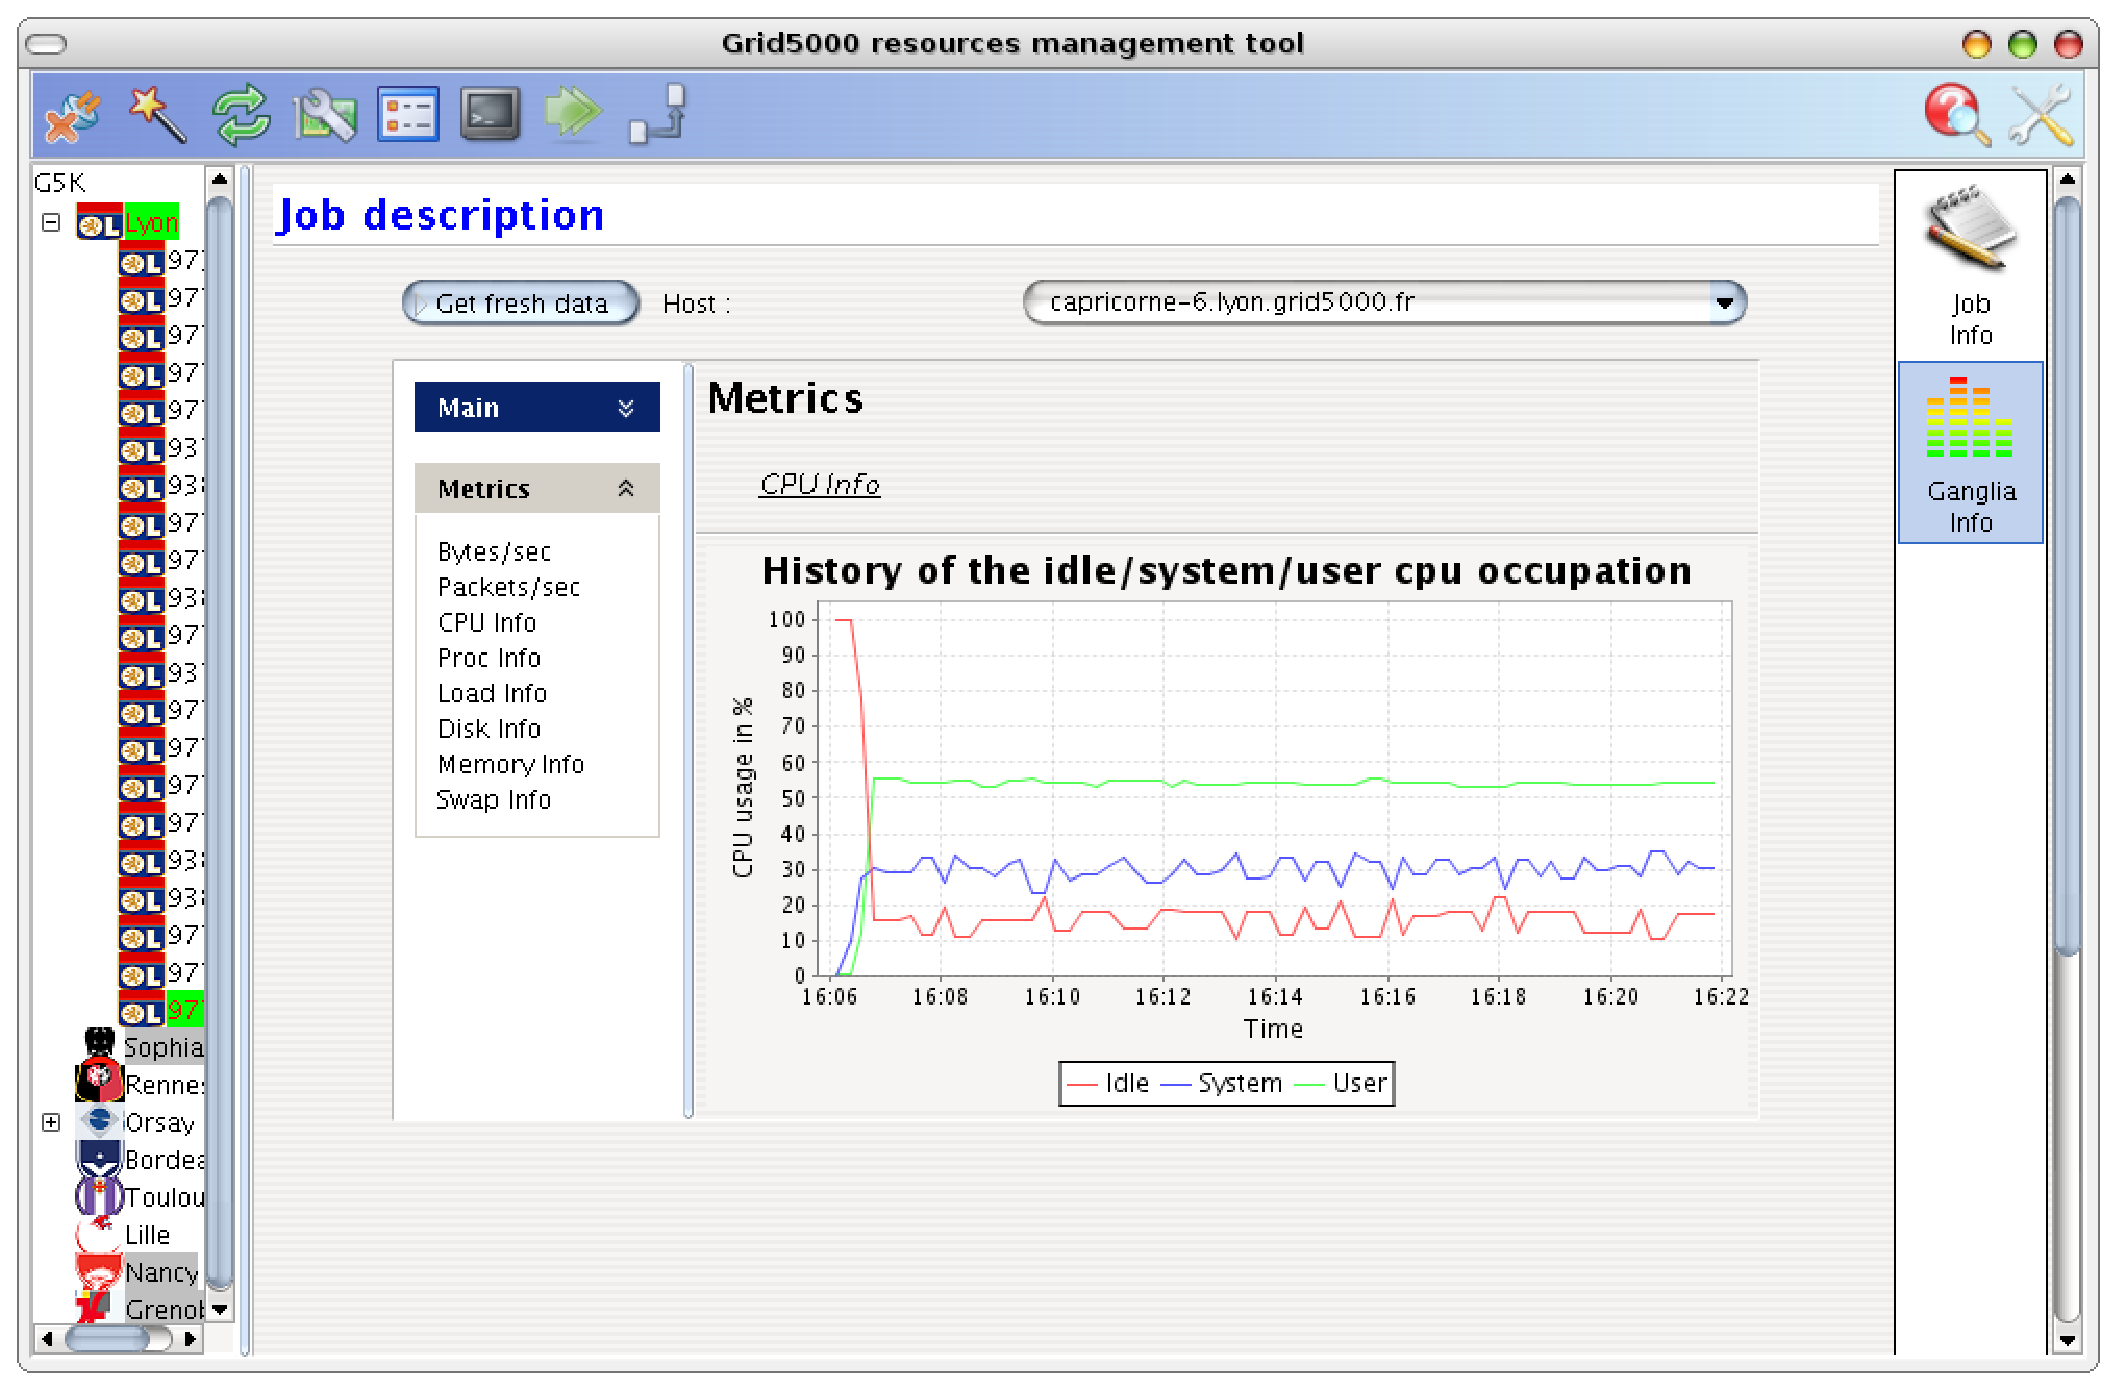
\includegraphics[width=0.5\linewidth]{figures/GRUDU_interface4_ganglia.eps}
  \caption{Ganglia plugin for the job view}
	\label{fig:GRUDU_view_job_ganglia}
  \end{figure}

\end{itemize}

